\documentclass[
	12pt,
	oneside,
	bibliography=totocnumbered]{scrartcl}


\usepackage{amsmath}


% formatting the captions of figures
\usepackage[bf]{caption} % make headings boldfont

% for drawing :-)
\usepackage{tikz} 
\usetikzlibrary{backgrounds} % to have a background layer
\usepackage{xcolor} % defining my own colors
\usetikzlibrary{positioning} % arrows between nodes and relative positions
\usetikzlibrary{arrows}

% For drawing the frames of the images
\fboxsep=0.5mm%padding thickness
\fboxrule=0.5mm%border thickness

% for drawing from different lotteries (left/right)
\usepackage{xifthen}

% Define colors
\colorlet{sampleShade}{gray!40}  % shading of sample trials
\colorlet{choiceShade}{blue!40}  % shading of choice trials
\colorlet{choiceCol}{red!70} % color of chosen option



% Some variables for drawing
\newcommand\sideAdj{13}
\newcommand{\imgSize}{.2\textwidth}
\newcommand{\descrTextWidth}{4cm}

% For figures
\usepackage{graphicx}
\graphicspath{{./figures/}} % specify relative path with extra {}


% For references
\usepackage[
	backend=biber, % troubleshooting: http://tex.stackexchange.com/questions/154751/biblatex-with-biber-configuring-my-editor-to-avoid-undefined-citations
	style=numeric-comp]{biblatex}

\addbibresource{DFE_refs.bib}


% For hyperlinks in table of contents, and references
\usepackage{hyperref}
\hypersetup{
    colorlinks,
    citecolor=black,
    filecolor=black,
    linkcolor=black,
    urlcolor=black}


% General document info
\title{Terminating Information Search}
\author{Stefan Appelhoff}



%%%%%%%%%%%%%%%%%%%%%%%%%%%%%%%%%%%%%%%%%%%%%%%%%%%%%%%%%%%%%%


\begin{document}
\maketitle
\tableofcontents
\listoffigures



\section{Introduction}

As agents in different environments, humans often find themselves in situations that require decisions based on limited knowledge about the available choice options. The topic of the present project is the process, how humans selectively sample choice options to arrive at a more refined knowledge about the properties of the options. Specifically, the interest lies in self-directed information search in sequential decision making problems. A short example illustrates the topic further: 

\begin{quotation}
Imagine that your laptop is broken and you want to acquire a new one. In the process, you may sequentially sample several available models and their respective properties such as prices, specifications, and reviews. To avoid indefinite browsing, you will need to terminate your search at some point and select a new laptop - most likely without having obtained full certainty about the best option.
\end{quotation} 

For the project described here, the aforementioned example will be transformed into an experimental paradigm that allows for the examination of behavioral and neural aspects of choice in a controled manner. Similar to the real life example, the experimental paradigm exhibits the following characteristics:

\begin{itemize}
\item There is an environment in which several options exist that will yield outcomes upon selection.
\item There exists limited knowledge about the options and the frequencies of their associated outcomes.
\item There will be the opportunity to obtain information about the options through a sampling of the options.
\item The overall goal is to maximize the positive outcomes obtained from the options in the long run.
\end{itemize}

In the paradigm, participants will make sequential decisions about which option to sample. In these trial to trial decisions, the question of interest to this project lies in how participants set their termination criteria. I.e., when do participants decide to terminate the information search in one option and switch to search another option? When do participants decide to stop sampling altogether and decide for one final option to be optimal based on current knowledge? The remainder of this document will be a concise formulation of the research questions followed by an outline of the experimental paradigm. Finally, the implementation of the experimental paradigm on a computer program will be described.


\section{Research Questions}

% Listing the research questions
\begin{enumerate}
\item How are sampling efforts sequentially allocated to the different options?
\item How do we arrive at a decision to terminate the information search?
\item What is the quantitative link between neural signals obtained by EEG with the behavioral data of participants performing the experimental paradigm.
\end{enumerate}



\section{The Experimental Paradigm}
The proposed experiment will be based on a combination  of two different paradigms that are well known in the literature.

\begin{enumerate}
\item The n-armed Bandit Paradigm
\item The Sampling Paradigm
\end{enumerate}

In the following, these two paradigms will be descibed in detail. Figure \ref{fig:paradigms} provides an overview of the paradigms. Afterwards, the combination of both paradigms for the present experiment will be outlined.


% Start the paradigm figure
% -------------------------------------------------
% -------------------------------------------------


% we want random values
\pgfmathsetseed{9999}
\pgfmathdeclarerandomlist{badLottery}{{0}{0}{0}{0}{0}{0}{0}{1}{1}{1}}
\pgfmathdeclarerandomlist{goodLottery}{{1}{1}{1}{1}{1}{1}{1}{0}{0}{0}}


\begin{figure}[t]
\begin{center}
\resizebox{.9\linewidth}{!}{%
\begin{tikzpicture}

% --------------------------------------------------%
%		 Begin with a general case   			   %
% --------------------------------------------------%


% TO DO

% figure part indication
\node [scale=1.5]at (0,20) {\textbf{A)}};

% drawing two initial rectangles as environment
\filldraw [color=black, fill=white](4,15) rectangle (5,16)node[above, scale=1.5]{\textbf{Environment}};
\filldraw [color=black, fill=white](5,15) rectangle (6,16);


% now "left choice" rectangles
\filldraw [color=black, fill=choiceCol](10,17) rectangle (11,18)node[above, scale=1.5]{\textbf{Choose Left}};
\filldraw [color=black, fill=white](11,17) rectangle (12,18);


% now "right choice" rectangles
\filldraw [color=black, fill=white](10,13) rectangle (11,14) node[above, scale=1.5]{\textbf{Choose Right}};
\filldraw [color=black, fill=choiceCol](11,13) rectangle (12,14);



\begin{scope}[on background layer]
% Drawing lines to the choice rectangles
\draw [line width=0.5mm](6,15.5) -- (10.01,17.5);
\draw [line width=0.5mm](6,15.5) -- (10.01,13.5);

% Drawing lines to outcome probabilities 
\draw [line width=0.5mm](12,13.5) -- (16,14.5) node[right, scale=1.5]{$\Pr({1 \mid right})=0.3$};
\draw [line width=0.5mm](12,13.5) -- (16,12.5)node[right, scale=1.5]{$\Pr({0 \mid right})=0.7$};

\draw [line width=0.5mm](12,17.5) -- (16,18.5)node[right, scale=1.5]{$\Pr({1 \mid left})=0.7$};
\draw [line width=0.5mm](12,17.5) -- (16,16.5)node[right, scale=1.5]{$\Pr({0 \mid left})=0.3$};

\end{scope}

% --------------------------------------------------%
%		 Continue with the Bandit Paradigm 		   %
% --------------------------------------------------%



% figure part indication
\node [scale=1.5]at (0,10) {\textbf{B)}};

% figure label
\node [scale=1.5, fill=choiceShade, right] at (8,8) {\textbf{Choice}};

% "direction of time"
\draw [line width=0.5mm,->] (8,8.8) -- (4,0) node [below,scale=1.5] {\textbf{Time}};

% the variables for all rectangles	
\foreach \x/\y/\filColLeft/\filColRight/\labelColLeft/\labelColRight/\action in {
4/8.8/choiceCol/white/black/white/left,
3.5/7.7/choiceCol/white/black/white/left, 
3/6.6/choiceCol/white/black/white/left, 
2.5/5.5/choiceCol/white/black/white/left, 
2/4.4/choiceCol/white/black/white/left, 
1.5/3.3/white/choiceCol/white/black/right, 
1/2.2/choiceCol/white/black/white/right, 
0.5/1.1/white/choiceCol/white/black/right, 
0/0/white/choiceCol/white/black/right}
{

% Draw a random number based on action
\ifthenelse{\equal{\action}{left}}{\pgfmathrandomitem{\outcome}{goodLottery}}{\pgfmathrandomitem{\outcome}{badLottery}};

% background shading
\begin{scope}[on background layer]
\fill [fill=choiceShade](\x-0.15,\y-0.15) rectangle (\x+2.15,\y+1.15);
\end{scope}

% all rectangles in a loop
\filldraw [color=black, fill=\filColLeft](\x,\y) rectangle (\x+1,\y+1) node[midway, color=\labelColLeft] {\textbf{\outcome}};

\filldraw [color=black, fill=\filColRight](\x+1,\y+1) rectangle (\x+2,\y) node[midway, color=\labelColRight] {\textbf{\outcome}};

}

%--------------------------------------------------%
%	      Now the Sampling Paradigm 			      %
%--------------------------------------------------%


% figure part indication
\node [scale=1.5]at (0+\sideAdj,10) {\textbf{C)}};

% figure labels
\node [scale=1.5, fill=sampleShade,right]at (8+\sideAdj,8) {\textbf{Sampling}};

\node [scale=1.5, fill=choiceShade,right]at (5+\sideAdj,1) {\textbf{Choice}};

% direction of time
\draw [line width=0.5mm,->] (8+\sideAdj,8.8) -- (4+\sideAdj,0) node [below,scale=1.5] {\textbf{Time}};

	
% the variables for all rectangles	
\foreach \x/\y/\filColLeft/\filColRight/\labelColLeft/\labelColRight/\action in { 
4+\sideAdj/8.8/choiceCol/white/black/white/left,
3.5+\sideAdj/7.7/white/choiceCol/white/black/right,
3+\sideAdj/6.6/white/choiceCol/white/black/right,
2.5+\sideAdj/5.5/white/choiceCol/white/black/right,
2+\sideAdj/4.4/choiceCol/white/black/white/left,
1.5+\sideAdj/3.3/white/choiceCol/white/black/left,
1+\sideAdj/2.2/choiceCol/white/black/white/left}
{

% Draw a random number based on action
\ifthenelse{\equal{\action}{left}}{\pgfmathrandomitem{\outcome}{goodLottery}}{\pgfmathrandomitem{\outcome}{badLottery}};


% background shading
\begin{scope}[on background layer]
\fill [fill=sampleShade](\x-0.15,\y-0.15) rectangle (\x+2.15,\y+1.15);
\end{scope}

% drawing all the rectangles
\filldraw [color=black, fill=\filColLeft](\x,\y) rectangle (\x+1,\y+1) node[midway, color=\labelColLeft] {\textbf{\outcome}};

\filldraw [color=black, fill=\filColRight](\x+1,\y+1) rectangle (\x+2,\y) node[midway, color=\labelColRight] {\textbf{\outcome}};

}


% drawing the choice rectangles
\filldraw [color=black, fill=choiceCol](0+\sideAdj,0) rectangle (\sideAdj+1,1) node[midway, color=black] {\textbf{1}};

\filldraw [color=black, fill=white](\sideAdj+1,1) rectangle (\sideAdj+2,0) node[midway, color=white] {\textbf{1}};

% background shading of choice rectangle
\begin{scope}[on background layer]
\fill [fill=choiceShade](\sideAdj-0.15,-0.15) rectangle (\sideAdj+2.15,1.15);
\end{scope}

%--------------------------------------------------%
\end{tikzpicture}
} % closing bracket from scaling

\captionsetup{width=.9\linewidth, format=plain}
\caption[Experimental Paradigms]{\textbf{A)} Depiction of a two-armed bandit. Note that the number of options in the environment can be extended arbitrarily to form an n-armed bandit. Each option contains its own probability mass function (pmf) of outcomes. These pmfs are unknown to a subject performing the bandit task. \textbf{B)} A typical run of trials in a bandit task. A subject sequentially chooses among options and is provided with feedback. Each trial represents a exploration-exploitation problem.  \textbf{C)} A typical run of trials in the sampling paradigm. A subject is allowed to sample the available options without an impact of the outcomes on the final payoff. At some point, the subject can decide to terminate sampling and choose one of the options, which will impact the final payoff. In the sampling paradigm, exploration and exploitation are thus distinct.}
\label{fig:paradigms}
\end{center}
\end{figure}
% -------------------------------------------------
% -------------------------------------------------

\subsection{The n-armed Bandit Paradigm}

The n-armed bandit paradigm was first formalized by Robbins in 1952 \cite{robbins1952}. It has since been the subject of interest in a variety of fields, see \cite{berry1985} for a review. Generally, participants are presented with n action that represent initially unknown outcome distributions with a set number of outcomes. Upon selection of an action, an outcome is yielded from the distribution and presented to the participant as a feedback. With this gained knowledge, the participant may continue with selecting the same or a different action. \\

The bandit paradigm offers a concise framework to study the exploration exploitation tradeoff common to the field of reinforcement learning. Here, exploration represents the goal to gather information about actions and their associated outcomes, while exploitation represents the goal to make use of the acquired information. A player who only explores will never exploit upon the accumulated knowledge, while a player who only exploits will most likely select suboptimal actions based on the inadequate knowledge about all actions. Hertwig \& Erev label the bandit paradigm as Partial-Feedback-Paradigm \cite{hertwig2009}.



\subsection{The Sampling Paradigm}

The sampling paradigm is similar to the bandit paradigm. The main difference is that exploration and exploitation are separated. This is achieved through permitting a participant to sample all actions without consequences for as long as the participant wishes. This stage represents purely the exploration, because the outcomes do not count towards a payoff. Once the participant decides to terminate the sampling process, there is one last opportunity to select any action. For this last choice, the outcome will affect the payoff and thus, this stage represents purely the exploitation. For more information, see \cite{hertwig2011, erev2014, hertwig2009}




\subsection{Combination of the Two Paradigms}

In the present project, we will apply a paradigm that combines the aforementioned bandit and sampling paradigms into a single experimental flow. We will further introduce another factor, namely the mode of interaction of the participant with the paradigm. Each of the factors will have two levels. In brief, we are thus talking about a 2x2 factorial design of an experiment as visualized in figure \ref{fig:design}. The two factors are:
\begin{itemize}
\item Paradigm condition
\item Interaction condition
\end{itemize}

\subsubsection{Paradigm condition}
The paradigm condition is governed by the bandit or sampling paradigm as the two levels respectively. Thus in the bandit condition, participants will perform a bandit task, whereas in the sampling condition, participants will perform a sampling paradigm task. This will allow us to uncover potential differences in behavior when humans are faced with a task that either combines or separates exploration and exploitation into stages.

\subsubsection{Interaction condition}
The interaction condition is goverened by active or passive interaction respectively. During the active condition, participants will actively select the actions and steer the flow of the paradigm. During the passive condition, participants will merely watch a replay of previous games. This allows us to make a distinction between (a) cognitive and motor involvement in active tasks and (b) neither cognitive nor motor involvement in the passive tasks. During the passive tasks there is no cognitive involvement, because participants are not solving or learning the underlying decision paradigm.

\subsubsection{Orthogonal task}
To make sure that participants pay attention even during the passive conditions, we introduce an orthogonal task to the 2x2 experimental design. Here, participants will have to react to a stimulus of a different color by a quick button press. If the reaction times are too slow, we can assume that the participants did not pay sufficient attention.

% 2x2 design figure
\begin{figure}[ht]
\begin{center}
\resizebox{.9\linewidth}{!}{%
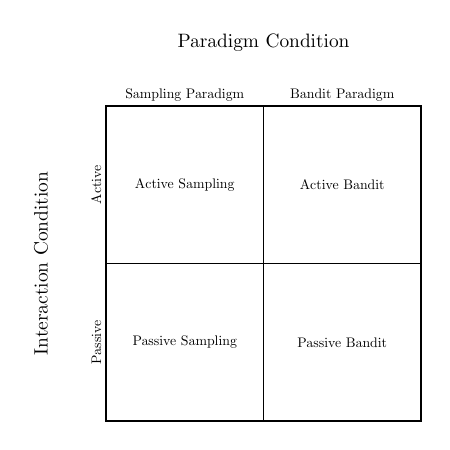
\begin{tikzpicture}


\draw (0,0) rectangle (2,2) node[scale=0.5,midway] {Passive Sampling};
\draw (2,0) rectangle (4,2) node[scale=0.5,midway] {Passive Bandit};
\draw (0,2) rectangle (2,4) node[scale=0.5,midway] {Active Sampling};
\draw (2,2) rectangle (4,4) node[scale=0.5,midway] {Active Bandit};

\node at (2,5) [scale=0.7,below] {Paradigm Condition};
\node at (1,4) [scale=0.5,above] {Sampling Paradigm};
\node at (3,4) [scale=0.5,above] {Bandit Paradigm};

\node at (-1,2) [scale=0.7,rotate=90,anchor=north, below] {Interaction Condition};
\node at (0,3) [scale=0.5,rotate=90,anchor=north,above] {Active};
\node at (0,1) [scale=0.5,rotate=90,anchor=north, above] {Passive};


\end{tikzpicture}
} % closing bracket from scaling

\captionsetup{width=.9\linewidth, format=plain}
\caption[Experimental Design]{The 2x2 factorial design of the experiment.}
\label{fig:design}
\end{center}
\end{figure}




\section{Computerized Implementation of the Experiment}

\begin{enumerate}

\item \textbf{The GUI} \\
At the beginning of the experiment, a graphical user interface will pop up, inquiring about the following information:
\begin{itemize}
\item Subject ID
\begin{itemize}
\item The subject ID will have at least three digits so that participant one will be '001', participant 2 will be '002' and so on.
\end{itemize}
\item Stimulus color
\begin{itemize}
\item The stimulus color can be set to either 'blue' or 'red', this entry determines, which color the winning stimulus will be. The losing stimulus will be set to the opposite color (e.g., 'blue', if the selection was 'red').
\end{itemize}
\item Starting condition
\begin{itemize}
\item  Finally, the starting condition can be set to either 'sp', which stands for sampling paradigm, or 'pfp', which stands for partial feedback paradigm (i.e., bandit). The selected option will be the initial condition of the experiment starting with 'active' as the second factor. This will be followed by a replay of the selected option (i.e., passive condition), before the move goes to the remaining condition, again in the order active - passive.
\end{itemize}
\end{itemize}


\item \textbf{Instructions} \\
Right after the initial GUI, there will be a set of initial instructions. I.e., the outline of the overall paradigm. Furthermore there will be more instructions before each upcoming condition.


\item \textbf{Active PFP Conditions} \\ 
If we have 100 trials for this condition, there will be about 4 'games' with 25 trials each. For each game, the lottery locations will be shuffled, so each game presents a new learning situation. See figure \ref{fig:banditFlow} for an overview.
\begin{itemize}
\item 'The lotteries have been shuffled' screen  [1 sec.]
\item Trial counter current\_trial / overall\_trials [1 sec.]
\item Fixation cross 
\item Reaction by participant [left] or [right] key to mimic selection of left or right lottery
\item Fixation cross screen: delay before outcome of choice is presented [1 sec.]
\item Feedback displayed in form of stimulus (see figure \ref{fig:stimuli}) [1 sec.]
\item Continue with next trial counter until current\_trial == overal\_trials
\item Show the payoff for the currently finished game [1 sec.]
\item Ask the participant which lottery was deemed more profitable.
\item Then, next game of PFP. Start with 'lotteries shuffled' screen
\end{itemize}

\begin{figure}[ht]
\begin{center}
\resizebox{.9\linewidth}{!}{%
\begin{tikzpicture}


% Insert all the pictures
\node[inner sep=0pt] (lotShuffle) at (0,0)
    {\fcolorbox{blue}{blue}{
\includegraphics[width=\imgSize]{lotShuffle.jpg}}};

\node[inner sep=0pt] (trialCount) at (0,-4)
    {\fcolorbox{red}{red}{
\includegraphics[width=\imgSize]{pfpCounter.jpg}}};    

\node[inner sep=0pt] (fixcross) at (0,-8)
    {\fcolorbox{red}{red}{
\includegraphics[width=\imgSize]{fixcross.jpg}}};
    
\node[inner sep=0pt] (outcome) at (0,-12)
    {\fcolorbox{red}{red}{
\includegraphics[width=\imgSize]{outBlueRight.jpg}}};
 
\node[inner sep=0pt] (earn) at (0,-16)
    {\fcolorbox{blue}{blue}{
\includegraphics[width=\imgSize]{earnZero.jpg}}}; 
   
\node[inner sep=0pt] (prefLot) at (0,-20)
    {\fcolorbox{blue}{blue}{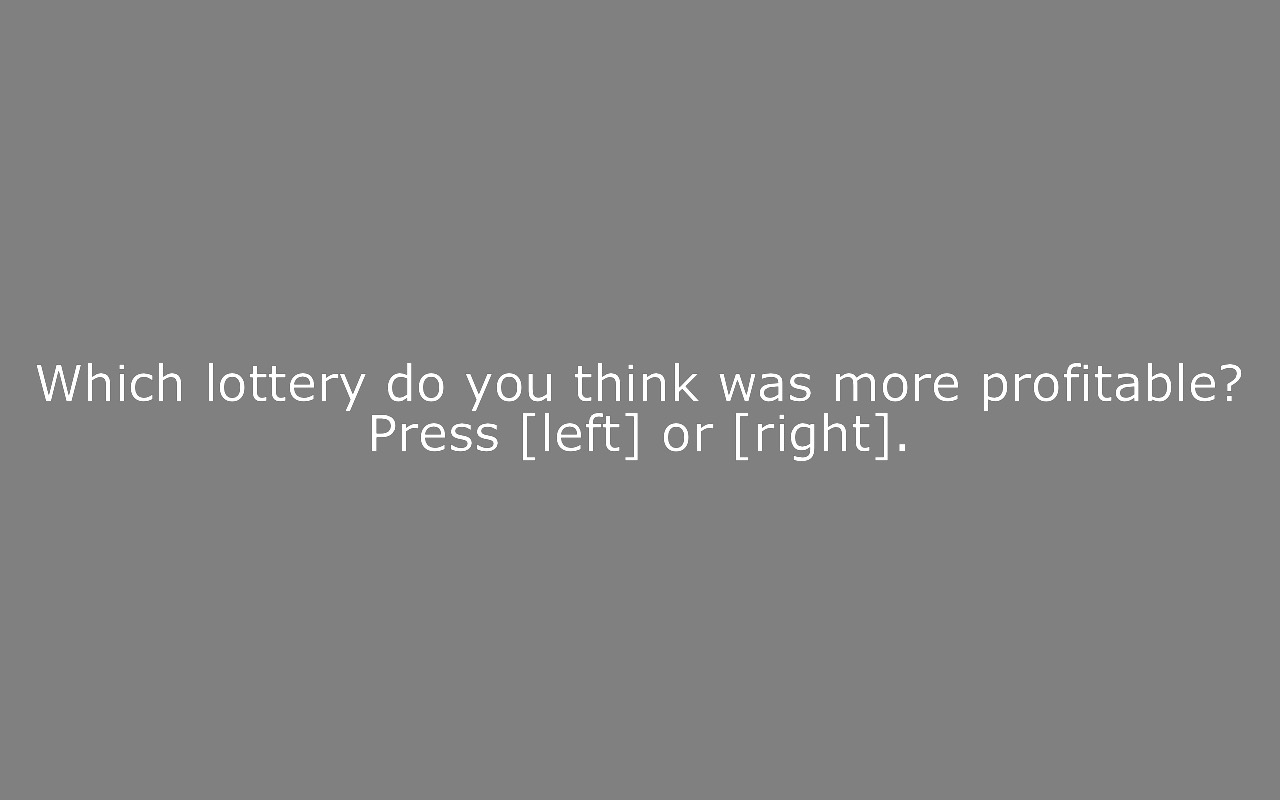
\includegraphics[width=\imgSize]{prefLot.jpg}}};



% Drawing all nodes between pictures
\draw[->,thick] (lotShuffle) -- (trialCount)
    node [midway,fill=white] {$1250\pm250$ ms};

\draw[->,thick] (trialCount) -- (fixcross)
    node [midway,fill=white] {$1250\pm250$ ms};
    
\draw[->,thick] (fixcross) -- (outcome)
    node [midway,fill=white] {t depends on RT};
    
\draw[->,thick] (outcome) -- (earn)
    node [midway,fill=white] {$1250\pm250$ ms};
    
\draw[->,thick] (earn) -- (prefLot)
    node [midway,fill=white] {$1250\pm250$ ms};
    

% Inserting describing text next to pictures

\node at (4,0) [text width=\descrTextWidth, align=left, right] {Options [left] and [right] are shuffled};

\node at (4,-4) [text width=\descrTextWidth, align=left, right] {Trial counter: Current trial of all trials in present game};

\node at (4,-8) [text width=\descrTextWidth, align=left, right] {Fixation cross: Participants select an option by clicking [left] or [right]};

\node at (4,-12) [text width=\descrTextWidth, align=left, right] {Outcome, or distractor, where participants need to press [space] as quickly as possible};

\node at (4,-16) [text width=\descrTextWidth, align=left, right] {Overall earnings are displayed};

\node at (4,-20) [text width=\descrTextWidth, align=left, right] {Participants are asked, which option they deemed more profitable};


% Drawing the bent arrows 
\draw[->,thick] (outcome.west) to [out=180,in=180] node[text width=0.2\textwidth, midway, fill=white, align=center]{$1250\pm250$ ms \\ Increment trial counter and repeat until max trial is reached} (trialCount.west) ;


\draw[->,thick] (prefLot.west) to [out=180,in=180] node[text width=0.2\textwidth, midway, fill=white, align=center] {t depends on RT \\ Increment game counter and repeat until max game is reached} (lotShuffle.west);


\end{tikzpicture}
} % close the resize box
\captionsetup{width=.9\linewidth, format=plain}
\caption[Flow Bandit Paradigm]{Experimental flow of the bandit paradigm. Red colors indicate the loop where participants explore and exploit there options. Once all trials have been spent within the red loop, a transition to the blue loop occurs, resetting the environment for a new game and leading to the red loop again, until all games are exhausted. Note: RT=Reaction time, ms=miliseconds, t=time}
\label{fig:banditFlow}
\end{center}

\end{figure}



\item \textbf{Passive PFP Condition} \\
\begin{itemize}
\item Replay of the Active PFP Condition
\item Take all timings as they were recorded before, and only interfere, when the timings are inadequately high or low. In these cases, we select a timing at random from the interval [0, 1] as implemented in matlab by: rand+rand.
\item Skip the question which lottery was deemed more profitable
\end{itemize} 


\item \textbf{Active SP Condition} \\
As opposed to the active PFP condition, we do not separate our overall 100 trials into distinct games. Instead, we will shuffle the lotteries after each 'choice' stage. Thus, there can be potentially many or few novel learning situations, depending on how often a participants picks 'choice' over 'continue to sample'.
\begin{itemize}
\item 'The lotteries have been shuffled' screen  [1 sec.]
\item Trial counter current\_trial [1 sec.]
\item Fixation cross 
\item Reaction by participant [left] or [right] key to mimic selection of left or right lottery
\item Fixation cross screen: delay before outcome of choice is presented [1 sec.]
\item Feedback displayed in form of stimulus (see figure \ref{fig:stimuli}) [1 sec.]
\item Question whether participant would like to: 
\begin{itemize}
\item Make a choice
\item Continue to sample
\end{itemize}
\item display choosen answer [0.7 sec.]
\item If 'continue to sample' was selected, continue with next trial counter else, present a choice screen.
\item Show the payoff for the currently finished game [1 sec.]
\item Then, continue with SP. Start with 'lotteries shuffled' screen
\end{itemize}


\begin{figure}[ht]
\begin{center}
\resizebox{.9\linewidth}{!}{%
\begin{tikzpicture}


% Insert all the pictures
\node[inner sep=0pt] (lotShuffle) at (0,0)
    {\fcolorbox{blue}{blue}{
\includegraphics[width=\imgSize]{lotShuffle.jpg}}};

\node[inner sep=0pt] (trialCount) at (0,-3)
    {\fcolorbox{red}{red}{
\includegraphics[width=\imgSize]{spCounter.jpg}}};    

\node[inner sep=0pt] (fixcross) at (0,-6)
    {\fcolorbox{red}{red}{
\includegraphics[width=\imgSize]{fixcross.jpg}}};
    
\node[inner sep=0pt] (outcome) at (0,-9)
    {\fcolorbox{red}{red}{
\includegraphics[width=\imgSize]{outRedLeft.jpg}}};
 
\node[inner sep=0pt] (question) at (0,-12)
    {\fcolorbox{red}{red}{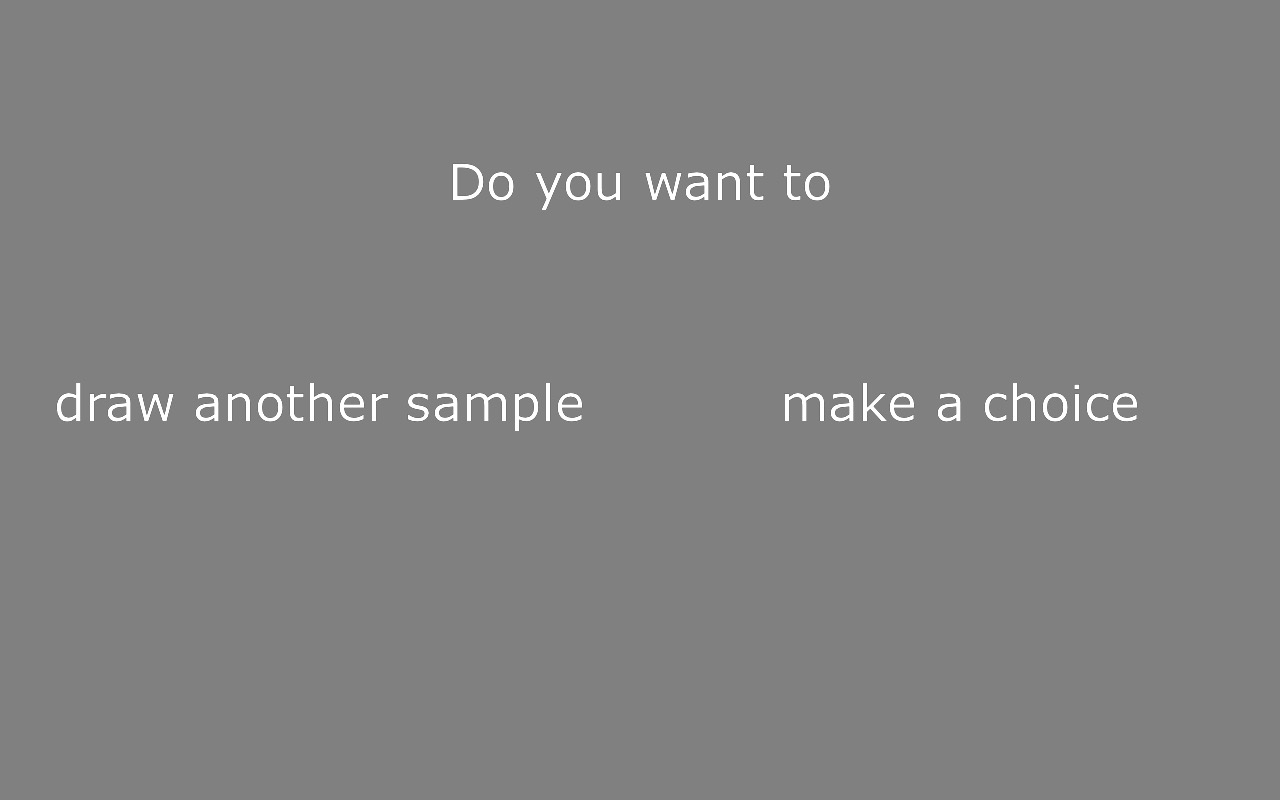
\includegraphics[width=\imgSize]{spQuestion.jpg}}}; 
   
\node[inner sep=0pt] (spQuestionSample) at (-4,-15)
    {\fcolorbox{red}{red}{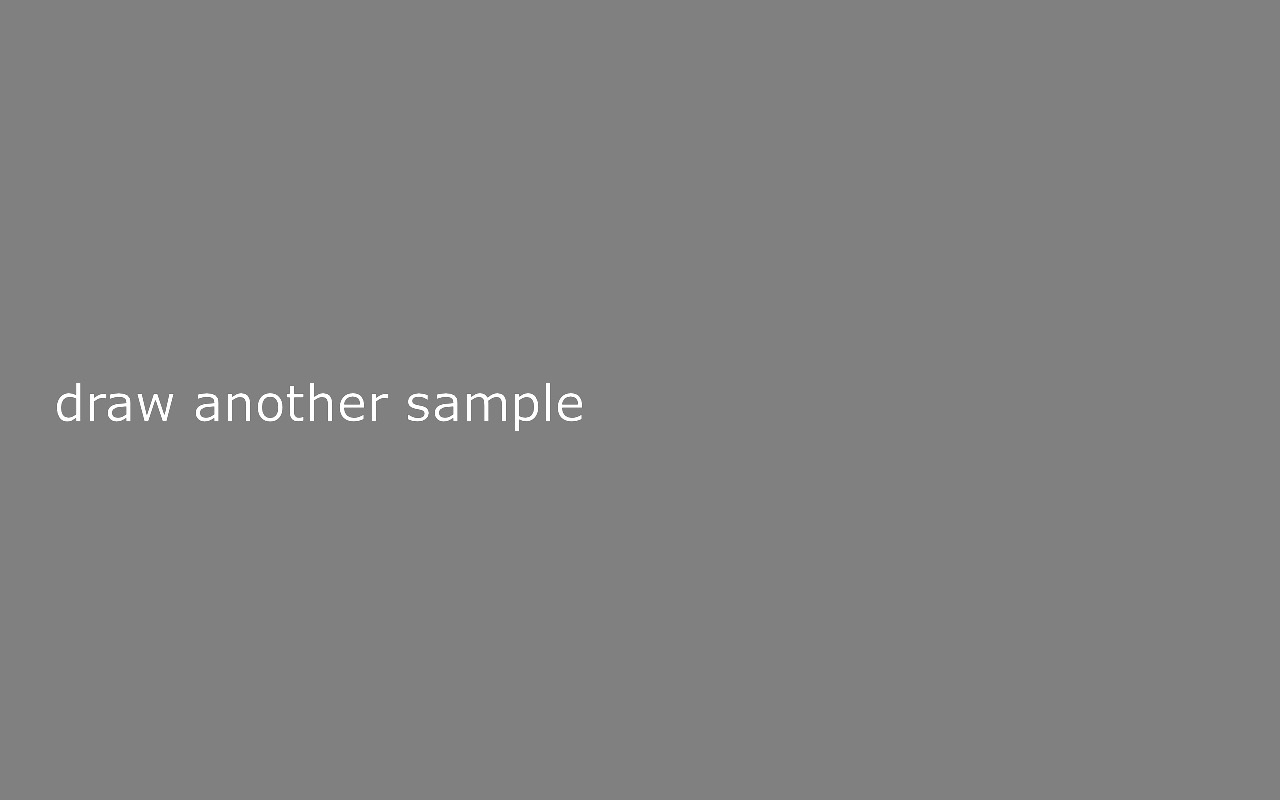
\includegraphics[width=\imgSize]{spQuestionSample.jpg}}};

\node[inner sep=0pt] (spQuestionChoice) at (4,-15)
    {\fcolorbox{blue}{blue}{
\includegraphics[width=\imgSize]{spQuestionChoice.jpg}}};

\node[inner sep=0pt] (noTrials) at (8,-15)
    {\fcolorbox{green}{green}{
\includegraphics[width=\imgSize]{spNoTrials.jpg}}}; 

\node[inner sep=0pt] (spChoice) at (4,-18)
    {\fcolorbox{blue}{green}{
\includegraphics[width=\imgSize]{spChoice.jpg}}};

\node[inner sep=0pt] (outcomeChoice) at (4,-21)
    {\fcolorbox{blue}{green}{
\includegraphics[width=\imgSize]{outBlueRight.jpg}}};
    
\node[inner sep=0pt] (earn) at (4,-24)
    {\fcolorbox{blue}{green}{
\includegraphics[width=\imgSize]{earnZero.jpg}}};






% Drawing all nodes between pictures
\draw[->,thick] (lotShuffle) -- (trialCount)
    node [midway,fill=white] {$1250\pm250$ ms};

\draw[->,thick] (trialCount) -- (fixcross)
    node [midway,fill=white] {$1250\pm250$ ms};
    
\draw[->,thick] (fixcross) -- (outcome)
    node [midway,fill=white] {t depends on RT};
    
\draw[->,thick] (outcome) -- (question)
    node [midway,fill=white] {$1250\pm250$ ms};

\draw[->,thick] (spQuestionChoice) -- (spChoice)
    node [midway,fill=white] {$750\pm250$ ms};
    
\draw[->,thick] (spChoice) -- (outcomeChoice)
    node [midway,fill=white] {$1250\pm250$ ms};

\draw[->,thick] (outcomeChoice) -- (earn)
    node [midway,fill=white] {$1250\pm250$ ms};



% Inserting describing text next to pictures

\node at (14,0) [text width=\descrTextWidth, align=left] {Options [left] and [right] are shuffled};

\node at (14,-3) [text width=\descrTextWidth, align=left] {Trial counter: Current trial only (no indication of maximum trials)};

\node at (14,-6) [text width=\descrTextWidth, align=left] {Fixation cross: Participants select an option by clicking [left] or [right]};

\node at (14,-9) [text width=\descrTextWidth, align=left] {Outcome of sampling, or distractor};

\node at (14,-12) [text width=\descrTextWidth, align=left] {Question whether to proceed with sampling (exploration) or make a choice (exploitation)};

\node at (14,-15) [text width=\descrTextWidth, align=left] {Quick show of selection};

\node at (14,-18) [text width=\descrTextWidth, align=left] {Which option to choose for exploitation};

\node at (14,-21) [text width=\descrTextWidth, align=left] {Outcome of choice};

\node at (14,-24) [text width=\descrTextWidth, align=left] {Earnings are displayed};





% describing text for double bent arrow
\node at (0,-15.2) [text width=\descrTextWidth, align=center] {t depends on RT};


% Drawing the bent arrows 

\draw[->,thick] (outcome.east) to [out=0, in=90] node [text width=0.2\textwidth, midway,fill=white] {If trial counter is at max, there is one last choice.} (noTrials.north);

\draw[->,thick] (noTrials.south) to [out=270, in=360] node [near start,fill=white] {t depends on RT} (spChoice.east);

\draw[->,thick] (question.south) to [out=270, in=180] node []{} (spQuestionChoice.west);    

\draw[->,thick] (question.south) to [out=270, in=0] node []{} (spQuestionSample.east);

\draw[->,thick] (spQuestionSample.north) to [out=90,in=180] node[text width=0.2\textwidth, midway, fill=white, align=center]{$750\pm250$ ms \\ Increment trial counter} (trialCount.west) ;

\draw[->,thick] (earn.east) to [out=0,in=0] node[text width=0.2\textwidth, near end, fill=white, align=center] {t depends on RT \\ Trial counter is not incremented. If trial counter at max, paradigm is stopped.} (lotShuffle.east);


\end{tikzpicture}
} % closing bracket from scaling

\captionsetup{width=.9\linewidth, format=plain}
\caption[Flow Sampling Paradigm]{Experimental flow of the sampling paradigm. Red colors indicate the sampling loop, from which one can transition to the blue choice loop, leading back to the sampling loop. Once the maximum of trials has been reached, a transition to the green loop for a last choice occurs. Note: RT=Reaction time, ms=miliseconds, t=time. }
\label{fig:spFlow}
\end{center}
\end{figure}




\item \textbf{Passive SP Condition} \\\item
\begin{itemize}
\item Replay of active SP condition
\item Timings are taken from active SP condition, unless they are inadequate (see also passive PFP condition)
\end{itemize}


\item \textbf{Orthogonal Task} \\
Throughout all four possible conditions, there will be a set chance (5\%) that instead of a blue or red stimulus, a green stimulus (\ref{fig:stimuli}) will occur. As soon as that stimulus is shown, participants ought to press the [space] key.
\end{enumerate} 








% Stimuli figure
\begin{figure}[t]
\begin{center}
\resizebox{.9\linewidth}{!}{%

\begin{tikzpicture}[even odd rule]


% Checkerboard for Stim 1: Red
\foreach \x in {0,...,7} \foreach \y in {0,...,7}
{
\pgfmathparse{mod(\x+\y,2) ? "red" : "white"}
\edef\colour{\pgfmathresult}
\path[fill=\colour] (\x,\y) rectangle ++ (1,1);
}


% Checkerboard for Stim2: Blue
\foreach \x in {11,...,19} \foreach \y in {0,...,7}
{
\pgfmathparse{mod(\x+\y,2) ? "blue" : "white"}
\edef\colour{\pgfmathresult}
\path[fill=\colour] (\x,\y) rectangle ++ (1,1);
}


% Checkerboard for Distractor Stim: Green
\foreach \x in {22,...,30} \foreach \y in {0,...,7}
{
\pgfmathparse{mod(\x+\y,2) ? "green" : "white"}
\edef\colour{\pgfmathresult}
\path[fill=\colour] (\x,\y) rectangle ++ (1,1);
}

% Putting a mask with circle-holes around it: Gray
\fill[fill=gray] (-1,-1) rectangle ++ (32,10) (4,4) circle (4cm) (15,4) circle (4cm) (26,4) circle (4cm);

\end{tikzpicture}
} % closing bracket from scaling

\captionsetup{width=.9\linewidth, format=plain}
\caption[Experimental Stimuli]{Three stimuli against a background as used in the experiment . The red and blue stimuli represent either a win or lose outcome. The green stimulus represents a distractor stimulus.}
\label{fig:stimuli}
\end{center}
\end{figure}

\clearpage
\printbibliography

\end{document}
